\documentclass[i1]{oss}
\setlength{\topmargin}{-.5in}
\setlength{\textheight}{9in}
\setlength{\oddsidemargin}{.100in}
\setlength{\textwidth}{6.25in}
\usepackage [dutch] {babel}
\usepackage{graphicx}
\usepackage{amsmath}
\usepackage{fullpage}
\usepackage{listings}
\usepackage{color}
\usepackage{soul}
\usepackage{gensymb}
\usepackage{caption}
\usepackage{subcaption}

\begin{document}

\team{6} % teamkleur
\members{Joren Verspeurt (r0258417)\\
         Sophie Marien (s0216517)\\
         Stef Noten (s0211264)\\
         Toon Nolten (r0258654) } % teamleden

\maketitlepage
\newpage
\tableofcontents
\pagebreak

\section*{Inleiding}

% Een inleiding: beschrijf hierin jullie algemene impressie van het systeem, de manier waarop
% jullie de analyse hebben aangepakt, etc.

In dit project moeten we JUnit ontleden via analyse tools die JUnit gaan visualiseren. JUnit is een testing en regressie testing framework in Java. Om beter de linken tussen de klassen te begrijpen werd er gebruik gemaakt van \emph{X-Ray} \cite{X-Ray} en \emph{AgileJ Structureviews} \cite{AgileJ Structureviews}. Hierna werd voor verdere analyse gebruik gemaakt van \emph{Design Pattern Detection Tool} \cite{Design Pattern Detection Tool} en \emph{CodeCity} \cite{CodeCity}. Voor de visualisatie van de klassendiagrammas en sequence diagrams werd er gebruik gemaakt van \emph{Visual Paradigm}.


\section{Ontwerpdocumentatie}

De klasse die de main methode bevat in het JUnit project is JUnitCore. JUnitCore is een facade voor het uitvoeren van testen. Via de run() methoden kunnen testen worden uitgevoerd. JUnitCore gebruikt de klasse Runner via de methode run(runner) die niet mag worden uitgevoerd. Deze wordt gebruikt bij het testen. De runner test en verwittigd de RunNotifier als er interessante gebeurtenissen voorvallen. 





\section{Evaluatie van het ontwerp}

%Een evaluatie van het ontwerp. Wat zijn sterke en zwakke punten van het ontwerp. Bespreek
%ook het gebruik (of het niet-gebruik) van patronen. Geef opnieuw sterke en zwakke punten
%van het ontwerp op dit vlak.

\section{Beschrijving van de analyse tools en evaluatie hiervan}

Voor de analyse van JUnit werden er vier analyse tools gebruikt. De verschillende tools zijn \emph{X-ray} \cite{X-Ray}, \emph{AgileJ Structureviews} \cite{AgileJ Structureviews} , \emph{Design Pattern Detection Tool} \cite{Design Pattern Detection Tool} en \emph{InFusion Hydrogen}. Om \emph{X-Ray} beter de begrijpen werd er ook nog gekeken naar \emph{CodeCity} \cite{CodeCity}.

\begin{description}

\item \emph{X-Ray}: \emph{X-Ray} is een visualisatie tool die de complexiteit van de klassen weergeeft. Figuur \ref{fig:X-Ray} geeft dit weer. De rechthoeken geven de klassen weer. De breedte van een rechthoek geeft het aantal methodes weer en de lengte het aantal lijnen code. Overerving wordt weergegeven via een boomstructuur. Met \emph{X-Ray }kan je ook opzoeken wie de parents zijn van een klasse of de childs. Via kleuren geven ze ook het type klasse mee: Abstract, Concrete, Interface en Internal Classes. Door een klasse te selecteren kan men de dependenties zien van deze klassen via rode lijnen die deze klasse verbind met de dependentie klassen. Het nadeel aan \emph{X-Ray} is dat de inkomende dependenties niet getoond worden, alleen de uitgaande dependenties.  \\
Via \emph{Codecity} hebben we meer inzicht gekregen in de afwezigheid van \emph{Godklassen} en ..

\begin{figure}[hb!]
	\centering
	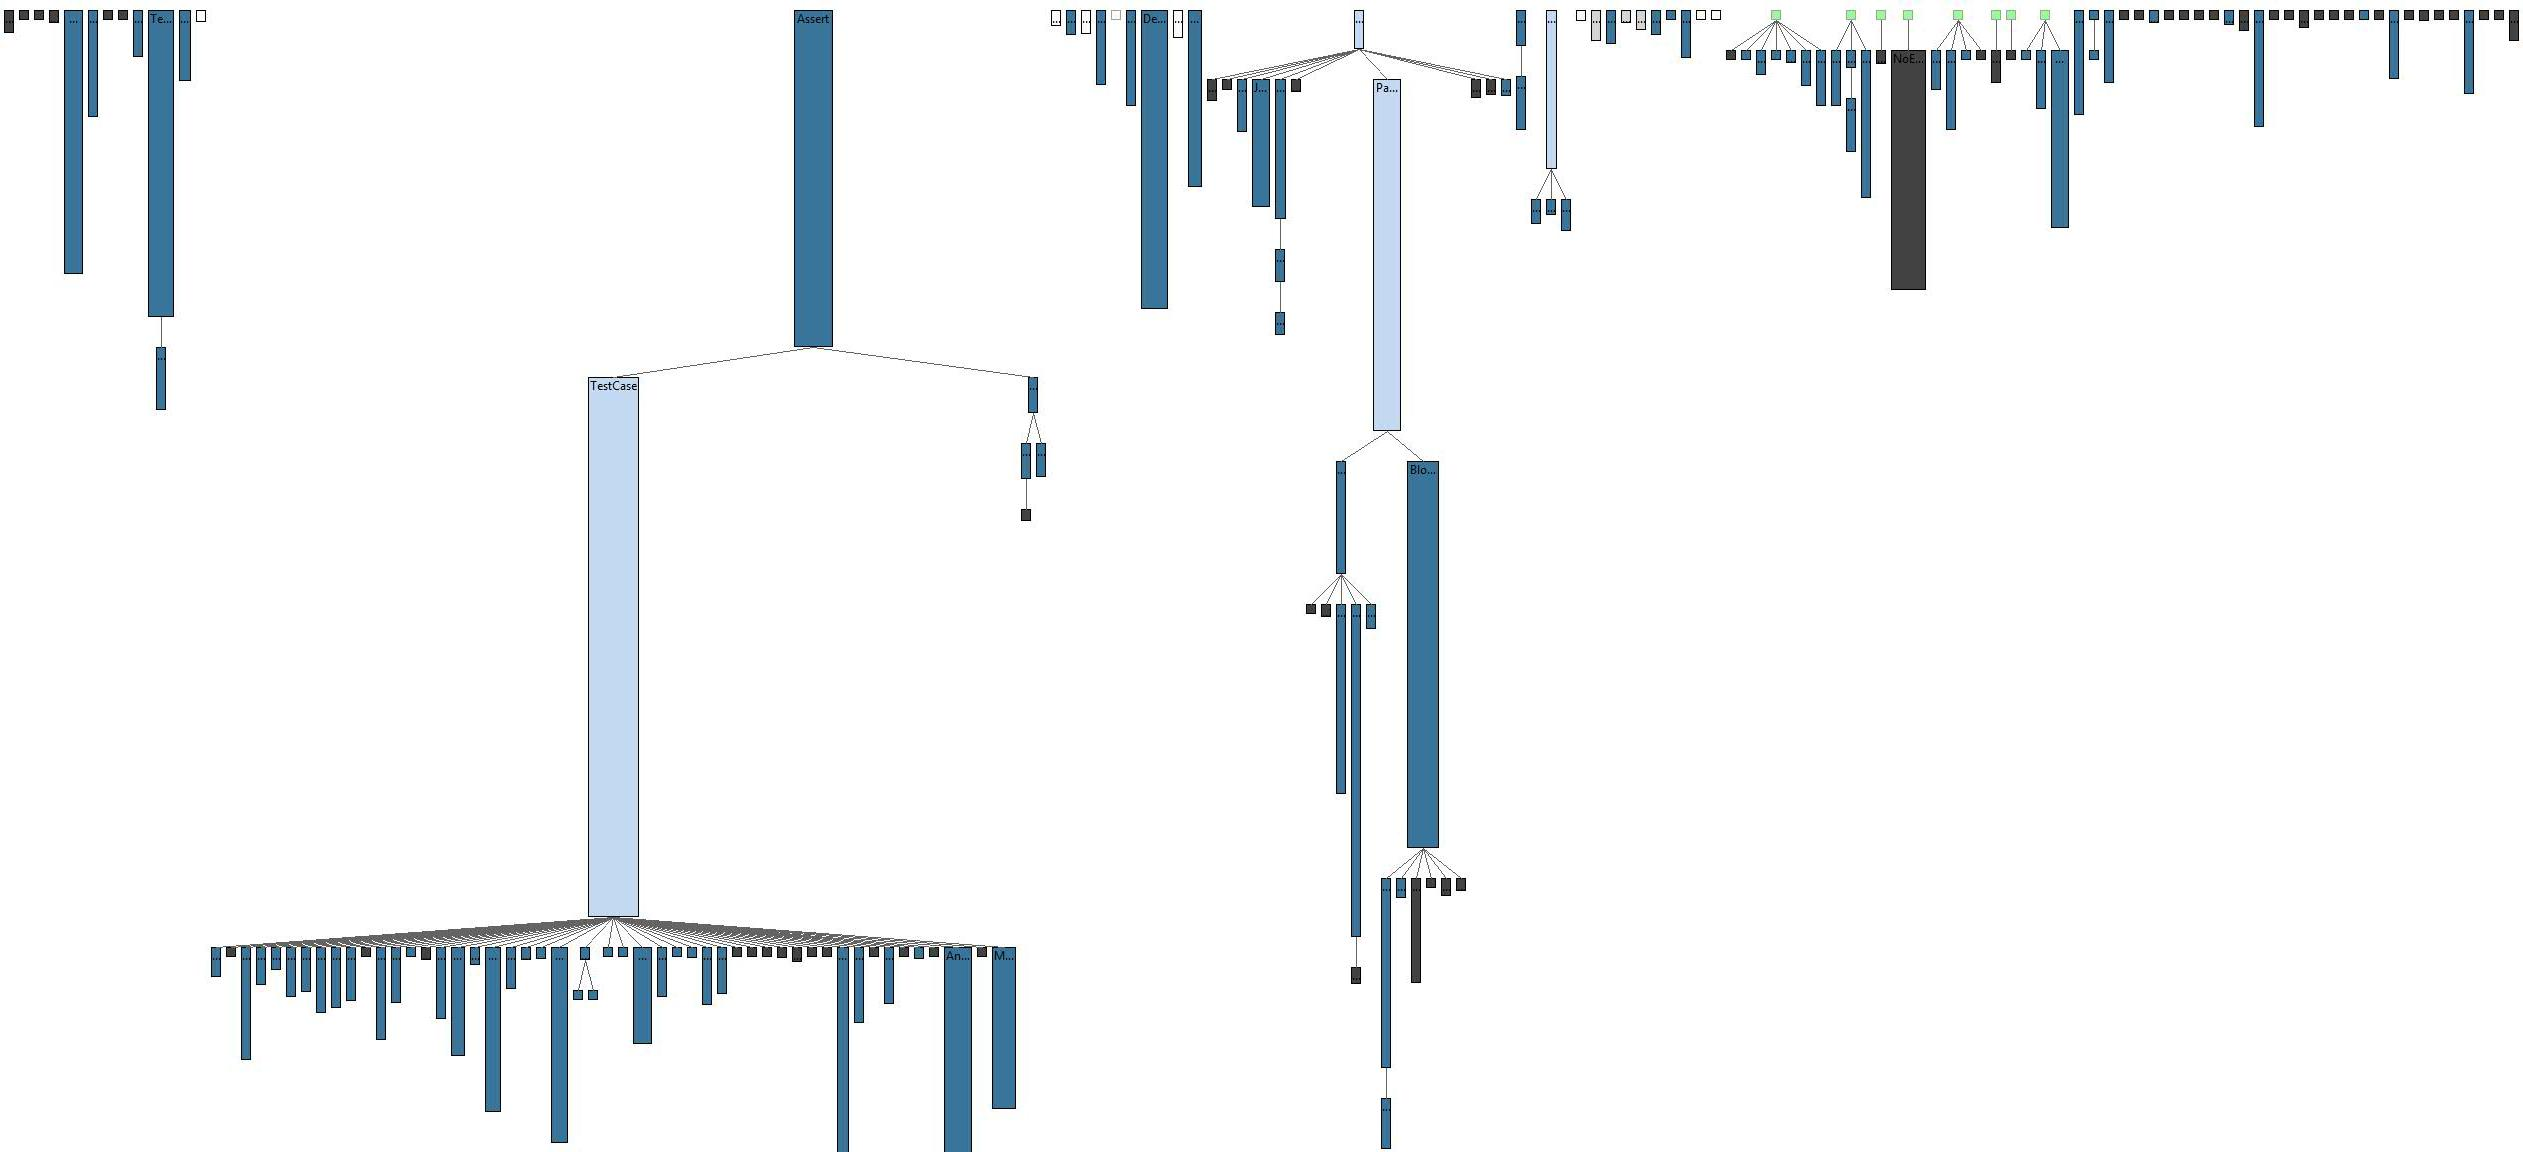
\includegraphics[width=0.65\textwidth]{XRayComplexity}
	\caption{X-Ray: Complexiteit}
	\label{fig:X-Ray}
\end{figure}

\item \emph{AgileJ Structureviews}: AgileJ Structureviews is een visualistatie tool die klassendiagrammas kan genereren. Figuur \label{fig:AgileJklassendia} geeft een voorbeeld visualisatie weer van een klassendiagramma die gegenereerd is via AgileJ.\\
Onze klassendiagrammas zijn gebaseerd op de klassendiagrammas die we via AgileJ gegenereert hebben. De klassendiagrammas die gegenereerd waren, bevatten alle methodes en velden waardoor het overzicht niet echt duidelijk was. Via filters konden deze methoden gefilterd worden. Ook kon er via de filters bepaald worden welke soort klasssen andere kleuren konden krijgen. AgileJ laat geen associaties zien, maar probeert dit te tonen door het aantal ... 


\begin{figure}[hb!]
	\centering
	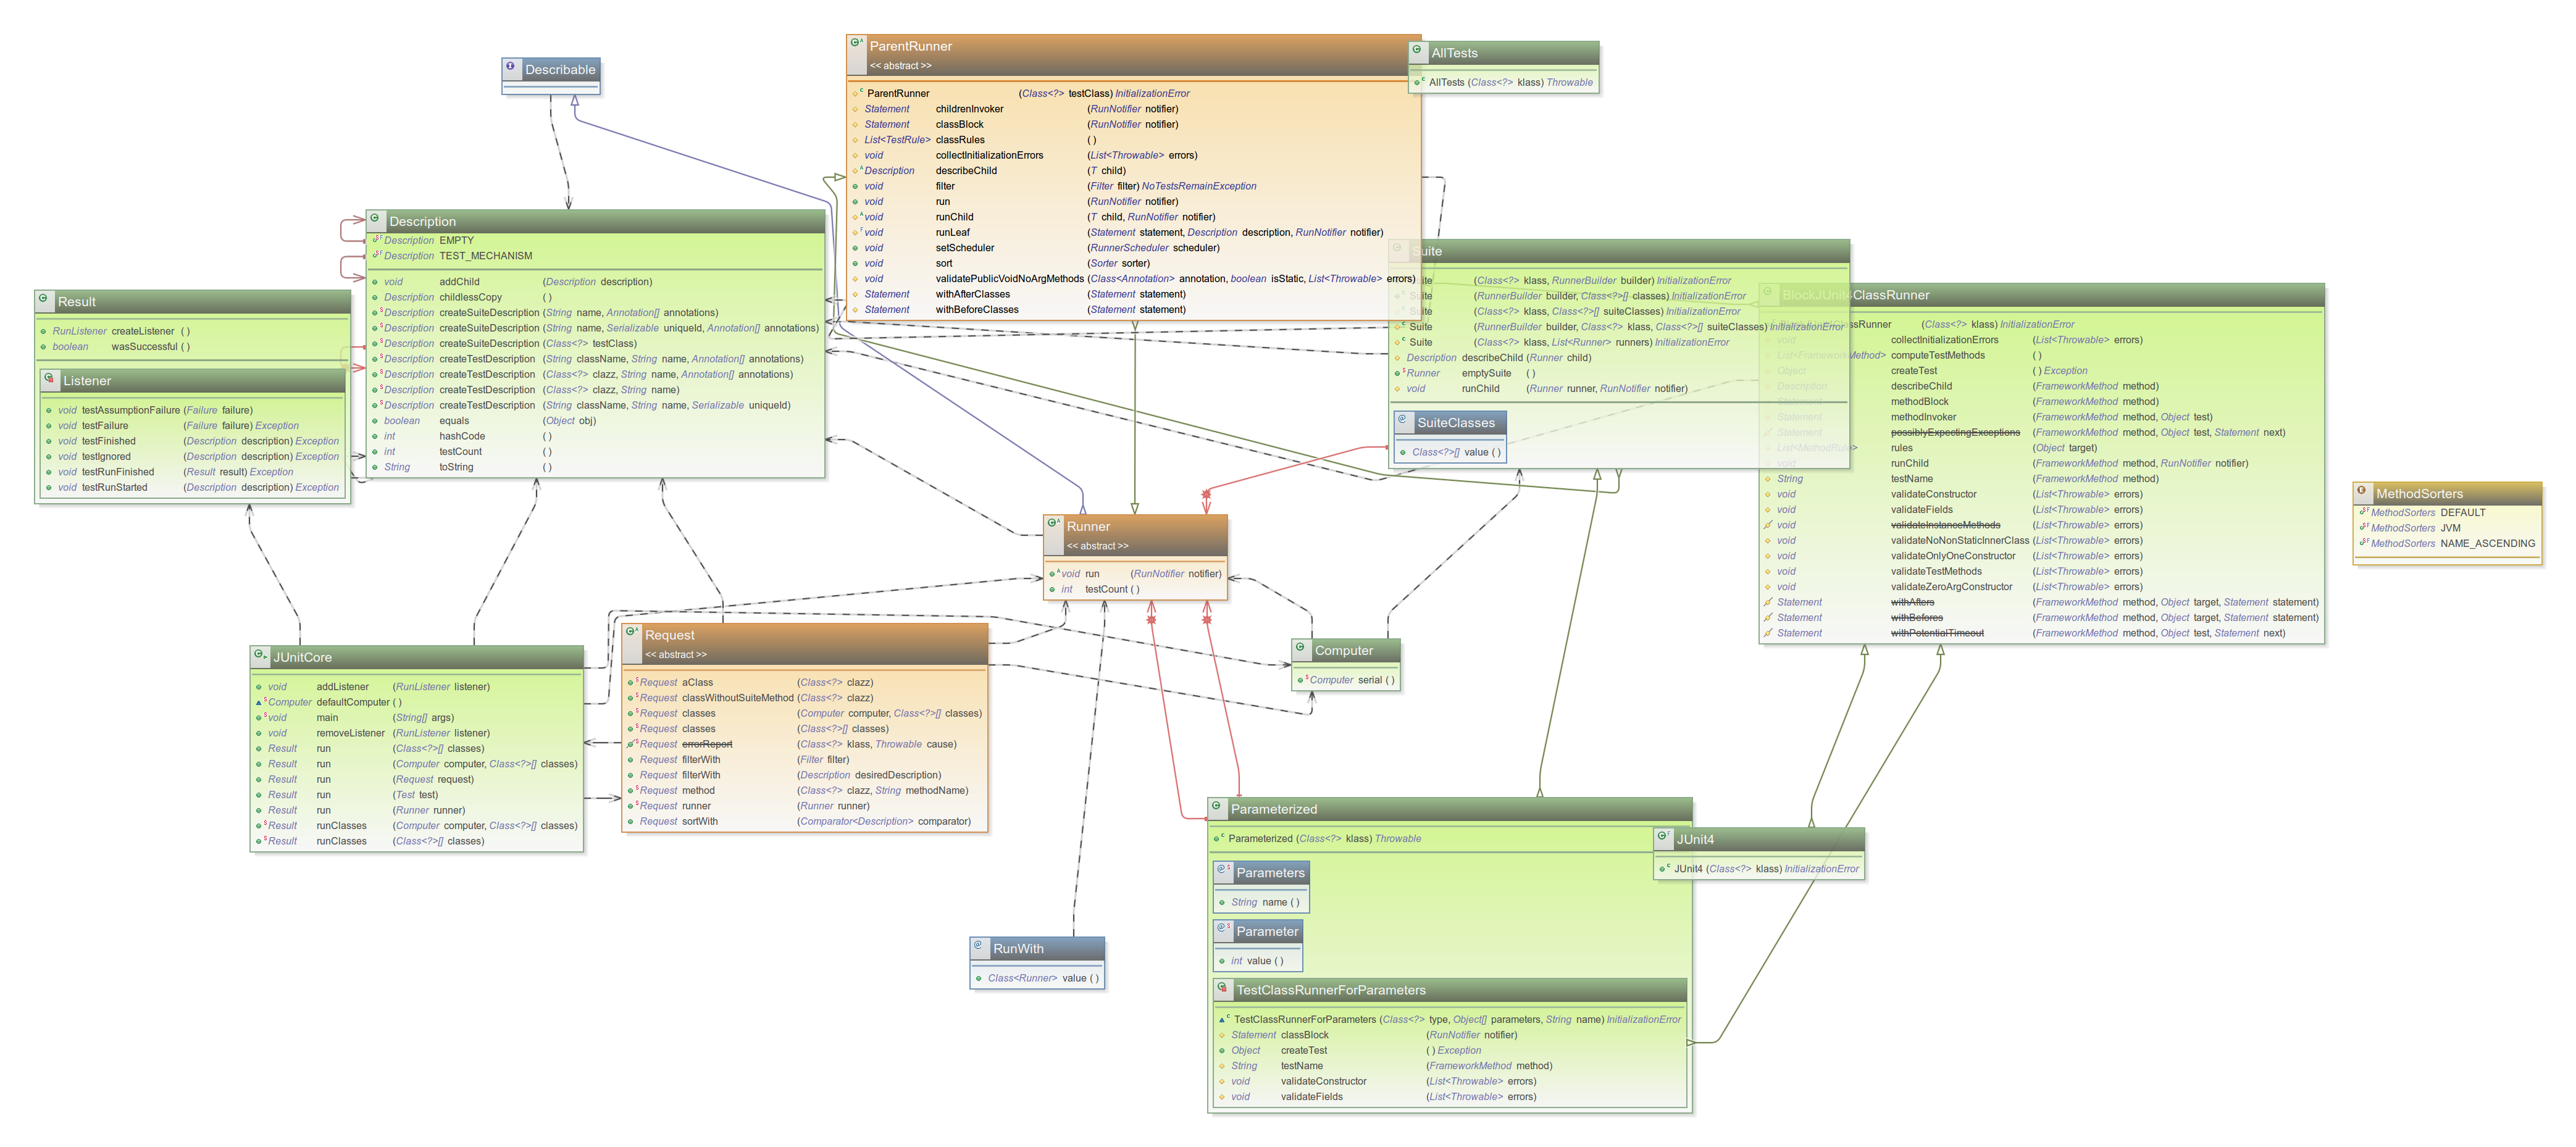
\includegraphics[width=0.65\textwidth]{AgileJKlassendiagramma}
	\caption{AgileJ Sturcutureviews: klassendiagramma}
	\label{fig:AgileJKlassendia}
\end{figure}

\item \emph{Design Pattern Detection Tool}: Design Pattern Detection Tool is een tool die het programma gaat checken op bepaalde patterns. Een overzicht van de patterns die gevonden zijn via de tool is te zien op de figuur \ref{fig:DesignPatterns}

\begin{figure}[hb!]
	\centering
	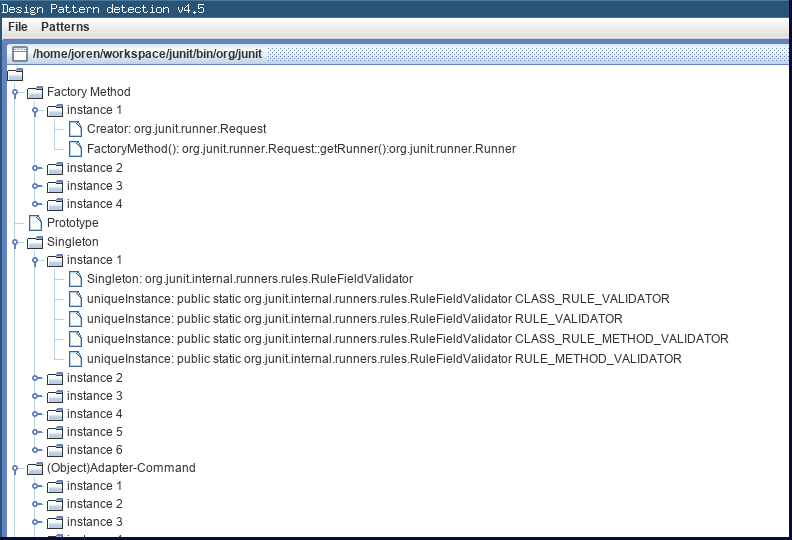
\includegraphics[width=0.65\textwidth]{Patterns1}
	\caption{Overzicht van de patterns}
	\label{fig:DesignPatterns}
\end{figure}

\item \emph{InFusion}: InFusion is een tool die een interpretatie geeft van het design van het programma en een overview pyramide kan opstellen die de interpretatie van de klassen hierarchies, de klassen en de methodes kan weergeven. Het genereert ook een design flaws perspective van het programma. Deze twee interpretaties zijn te zien op de figuur \ref{fig:InFusion}.

\begin{figure}
\centering
	\begin{subfigure}[h]{0.65\textwidth}
		\centering
		\includegraphics[width=\textwidth]{InFusion1}
		\caption{Overview Pyramid}
	\end{subfigure}
	\begin{subfigure}[h]{0.65\textwidth}
		\centering
		\includegraphics[width=\textwidth]{InFusion2}
		\caption{Design flaw perspective}
	\end{subfigure}
\caption{Screenshots van InFusion}
\label{fig:InFusion}
\end{figure}


\end{description}


\section{Analyse tools en belangrijke resultaten}
Agilj filters gebruikt, Codecity, Xray
Statements wordt gebruikt om alle annotaties uit te voeren
.runner en .runners

\section{Evaluatie testen}

\section{Samenvatting}

\section{Projectbeheer}

Wij zijn vrij laat begonnen aan het project omdat onze groep nog niet samengesteld was in het begin van de eerste week. In de eerste week zijn we samengekomen om samen de opdracht te lezen en de verschillende tools onder elkaar te verdelen. 

Er werd steeds in een tabel bijgehouden wie wanneer aan wat had gewerkt. Dit gaf eveneens een zicht op wat er al klaar was en wat nog moest gebeuren. \\
Tabel~\ref{tab:werkuren} geeft weer hoeveel tijd in het project gestoken werd. Figuur~\ref{fig:werkverdeling} toont wie aan welke aspecten van het project heeft gewerkt.

\newpage
\begin{flushleft}
\begin{thebibliography}{4}

\bibitem{X-Ray}
\emph{X-Ray}
\begin{scriptsize}
geraadpleegd op 11/10/2013 via: \mbox{http://xray.inf.usi.ch/xray.php} en \mbox{https://marketplace.eclipse.org/content/x-ray-software-visualization}
\end{scriptsize}

\bibitem{AgileJ Structureviews}
\emph{AgileJ Structureviews}
\begin{scriptsize}
geraadpleegd op 11/10/2013 via: \mbox{http://www.agilej.com/}
\end{scriptsize}

\bibitem{Design Pattern Detection Tool}
\emph{Design Pattern Detection Tool}
\begin{scriptsize}
geraadpleegd op 15/10/2013 via: \mbox{http://java.uom.gr/~nikos/pattern-detection.html} versie  Design Pattern detection Tool (version 4.5 - build 28/05/2010)
\end{scriptsize}

\bibitem{InFusion}
\emph{InFusion}
\begin{scriptsize}
geraadpleegd op 17/10/2013 via: \mbox{http://www.intooitus.com/products/infusion/download} versie InFusion Hydrogen v1.8.0
\end{scriptsize}

\bibitem{CodeCity}
\emph{CodeCity}
\begin{scriptsize}
geraadpleegd op 9/10/2013 via: \mbox{http://www.inf.usi.ch/phd/wettel/codecity.html} 
\end{scriptsize}

\end{thebibliography}
\end{flushleft}

\end{document}



